\chapter{Deus et Eliseus Ascenderunt in Caelum}
\begin{center}
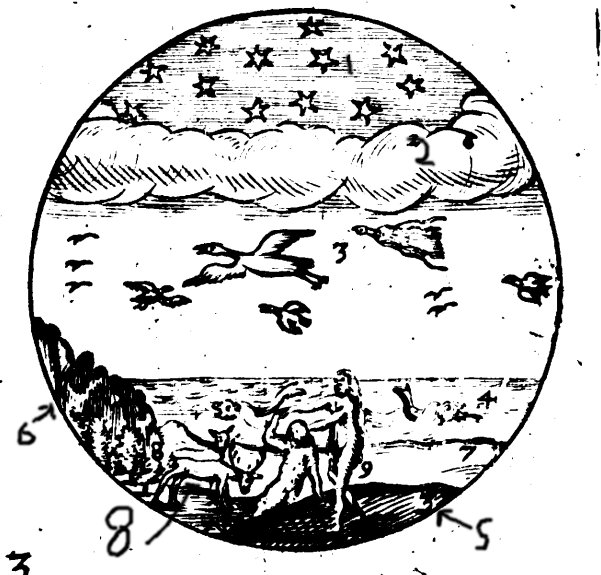
\includegraphics[scale=1.5]{World.png}
\end{center}

\section{Intended Audience}
This is intended for students who have completed Lectio 3 and 4 of Latin by the Natural Method and Chapter 4 of Lingua Latina Per Se Illustrata. 

\section{Text}
Deus et Eliseus filius meus parvus ascenderunt in Caelum. Quomodo Deus ascendit in caelum, si sine corpore et sine loco est? Deus incarnationem habet, qui ascendit in caelum et descendit ex caelo. Incarnatio secundi hypostasis trinitatis est Iesus Christus. Ergo, Deus (in incarnatione) et Eliseus fuerunt in nubibus, quia ascenderunt in Caelo. Elias etiam et Iesus ascenderunt in caelum, sed Iesus solus sedet ad manum dexteram Dei. 

In Caelo, Eliseus vidit aves, quae volaverunt per nubes. Ubiubi Avis volavit, movet aerem. Ubiubi Eliseus aspexit, Eliseus vidit aves et nubes. Quid non vidit Eliseus? Angelos non vidit Eliseus. Cur? Estne Angeli in Caelo cum Deo?  Angeli in caelo sunt. Caelum habet tres significationes. Significatio prima est haec \: Ubi sunt nubes et aves et sol et luna. Significatio secunda \: Ubi sunt Angeli. Angeli non habent corpora nec locos, sicut Deus in essentia, sed angeli in Caelo sunt. Tertia significatio est ubi est Deus, in aeterno. Angeli non sunt in aeterno, sed in aevo. Angeli in aevo sunt quia creationes immortales sunt sed non ex aeterno. Ubiubi es, Omnes Angeli illic sunt. Ubiubi es, Deus tenet te in ente et cum te est. 

Dicamus de significatione prima. Caelum rotatur et ambit terram statem in medio. Quid est "ambit". Sicut terra ambit solem, et nubes ambunt terram. Iesus filius Nun (Hic est Joshua anglice) ambit Jerichonem septies. Quid est "rotatur"? Terra rotatur et ambit Solem. Sol non rotatur, sed stat. Sol, ubiubi est, fulget perpetuo in terra. Si nox in Europa, dies in Asia. Nubes enim sunt in caelo, tamen sol fulget, sed radii non sunt in terra. Radius est lux quam misit Sol in terra. Eliseus non vidit solem, si in nubibus densis est. Eliseus autem vidit aves, ergo nubes densae non sunt. 


\footnote{\textbf{Montēs} = Montains or Hills}